\newpage
\thispagestyle{plain}

\section{Technická dokumentácia}\label{technical_documentation}

\subsection{Špecifikácia požiadaviek}

\paragraph{Nefunkčné požiadavky}

Na systém sú kladené nasledujúce nefunkčné požiadavky

\begine{itemize}
\item{\textbf{Rýchlosť} hlavným sledovaným parametrom pri webových aplikáciach 
    je čas načítania stránky, podľa štatistík, stránka ktorá sa načíta nad 2 sekundy 
    má veľkú pravdepodobnosť, že sa používateľ na ňu
    nevráti\footnote{http://www.mcrinc.com/Documents/Newsletters/201110\_why\_web\_performance\_matters.pdf},}
\item{\textbf{Bezpečnosť} je dôležitá najmä skrz to, že stránka bude profilovať používateľov,
    čo by sa mohlo dať zneužiť. Je potrebné použiť vhodný spôsob prihlasovania a 
    ukladania prihlasovacích údajov,}
\item{\textbf{Stabilita} aplikácia by mal vydržať fungovať dostačujúce časové obdobie bez výskytu
    väčšej chyby,}
\item{\textbf{Modularita} by mala byť zabezpečená pre prípad budúcich úprav aplikácie.}
\end{itemize}

Aplikácia by mala ďalej byť schopná správne pracovať na platforme PHP verzie vyššej ako 5.4
pričom je predpokladaná prítomnosť GD a mcrypt rozšírenia. Po vizuálnej stránke by sa aplikácia
mala dobre zobraziť vo všetkých moderných prehliadačoch a to responzívne. Ďalej aplikácia
bude potrebovať prítomnosť databázy MySQL verzie aspoň 5.1, prípadne PostrgreSQL.

\paragraph{Funkčné požiadavky}

Aplikácia bude poskytovať možnosť vyhľadania piesne, pričom bude 
následne poskytovať odporúčania, vďaka čomu umožní prieskumné vyhľadávanie.
Ďalej bude používateľovi umožňovať nechať si odporučiť dokumenty na základe 
ním zobrazených dokumentov a vytvorenie spevníka pre kombináciu niekoľkých 
používateľov.

Aplikácia bude mať tak isto administračné rozhranie, kde bude možné zobrazovať a
spravovať (mazať a upravovať) zaregistrovaných používateľov.

\subsection{Návrh projektu}

Projekt ja implementovaný v aplikačnom rámci Yii2. V rámci tohoto aplikačného rámca 
je použitých niekoľko návrhových vzorov. Základom je návrhový vzor
MVC\footnote{http://en.wikipedia.org/wiki/Model\%E2\%80\%93view\%E2\%80\%93controller}, 
ktorý následne na správu dát dopĺňa návrhovým vzorom
ActiveRecord\footnote{http://en.wikipedia.org/wiki/Active\_record\_pattern}, ktorý
slúži na prácu s dátami. Tak isto program umožňuje použiť buď LazyLoading\footnote{http://en.wikipedia.org/wiki/Lazy\_loading}, alebo 
EagerLoading\footnote{Pravý opak LazyLoading kedy je snaha vybrať všetky data z databázy naraz}.

Kód je napísaný tak, že každý objekt má vlastný súbor a zdrojové súbory sú rozdelené podľa
toho, čo reprezentujú (modely, pohľady, kontrolery, widgety, asety, komponenty, kravlery,
migracie a testy).

\subsection{Implementácia}

\paragraph{Funkcie v modeli dokumentu}

Tieto funkcie sa nachádzajú v súbore models/Document.php

\begin{lstlisting}[code=php,
caption=Funkcia na porovnanie dokumentu so sadou ováhovaných značiek]
public static function match($tags, $exclude = false) {
    $case = Globals::sqlCase($tags,'tag.name');

    $subQuery = (new Query)->select('id')
        ->from('tag')
        ->where(['name' => array_keys($tags)]);

    $query = (new Query)->select('document_id')
        ->from('map_document_tag map')
        ->innerJoin('tag', new Expression('tag.id = map.tag_id'))
        ->where(['tag_id' => $subQuery])
        ->groupBy('document_id')
        ->orderBy(new Expression("SUM(weight* $case ) DESC"))
        ->limit("50");

    if($exclude)
        $query->andWhere(['not in', 'document_id', $exclude]);

    return Document::find()->where(['id' => $query]);
}
\end{lstlisting}

\begin{lstlisting}[
    code=php,
    caption=Porovnanie dokumentu so sadou značiek\, akurát, že predpokladá identifikátor
    značiek namiesto mien
]
public static function matchIds($tags) {

    $case = Globals::sqlCase(ArrayHelper::map($tags, 'tag_id', 'weight'),'tag_id');

    return Document::find()
        ->innerJoin('map_document_tag map', 'map.document_id=document.id')
        ->where(['map.tag_id' => ArrayHelper::getColumn($tags, 'tag_id')])
        ->groupBy('document.id, document.name')
        ->orderBy(new Expression("SUM(weight * $case) DESC"));
}
\end{lstlisting}

\begin{lstlisting}[
code=php,caption=Funkcia, ktorá zoberie vyhľadávaciu frázu a vráti na základe nej dokumenty]
public static function search($query)
{
    $query_tags = array_count_values(Tag::escape($query));
    return self::match($query_tags);
}
\end{lstlisting}

\begin{lstlisting}[code=php,caption=Funkcia, ktorá vyhodnocuje typ značky na základe príznakov
DN - značka je názov dokumentu\, IN - značka je interpret dokumentu\, DT - značka sa nachádza
v názve dokumentu\, IT - značka sa nachádza v názve interpreta.]
public static function getTagType($IN, $DN, $IT, $DT) {
    if($DN && $IN) return 8;
    elseif($DN && $IT && !$IN) return 7;
    elseif($IN && $DT) return 6;
    elseif($DN) return 5;
    elseif($IN) return 4;
    elseif($DT && $IT) return 3;
    elseif($DT) return 2;
    elseif($IT) return 1;
    else return 0;
}
\end{lstlisting}

\begin{lstlisting}[
    code=php, caption=Funkcia, ktorá vráti spoločné značky dokumentov
    dokument1 a dokument2
]
public static function similiarTags($document1, $document2) {
    return Tag::find()
        ->innerJoin('map_document_tag map1', 'map1.tag_id=tag.id')
        ->where(['map1.document_id' => $document1->id])
        ->innerJoin('map_document_tag map2', 'map2.tag_id=tag.id')
        ->andWhere(['map2.document_id' => $document2->id])
        ->andWhere(new Expression('map1.document_id = map2.document_id'));
}
\end{lstlisting}

\begin{lstlisting}[
    code=php,
    caption=Funkcia vracajúca podobné dokumenty aktuálnemu dokumentu
]
public function getSimiliar() {
    return static::find()
        ->innerJoin('map_document_tag map1', 'map1.document_id=document.id')
        ->innerJoin('map_document_tag map2', ['AND',
                'map2.tag_id=map1.tag_id',
                ['map2.document_id' => $this->id],
                ['<>', 'map1.document_id', $this->id]
            ])
        ->groupBy('document.id')
        ->orderBy(new Expression('SUM(map1.weight * map2.weight) DESC'))
        ->having(new Expression('COUNT(*) > 1'));
}
\end{lstlisting}

\paragraph{Funkcie v modely používateľa}

Tieto funkcie sa nachádzajú v súbore models/User.php

\begin{lstlisting}[
    code=php,
    caption=Odporúčanie pre viacerých používateľov\, vráti ováhované značky
]
public static function recommendFor($ids) {
    $expression = new Expression(
        '((COUNT(DISTINCT user_id) / '.
        count($ids).'.00) * '.
        'LOG(COUNT(*) + 1))'
    );
    return (new Query())
        ->select(['tag_id', 'weight' => $expression])
        ->from('view')
        ->where(['user_id' => $ids])
        ->orderBy($expression)
        ->groupBy('tag_id');
}
\end{lstlisting}

\begin{lstlisting}[
    code=php,
    caption=Algoritmus, ktorý vráti dlhodobé zaujmy použitím delenia histórie na obdobia
]
public function getTimeAwareRecommendDocuments($exclude = false) {
        $view_count = View::find()->where(['user_id' => $this->id])->count();
    $per_cluster_top = 50 / Yii::$app->params['long_term_groups'];
    $cluster_size = floor(
        $view_count / Yii::$app->params['long_term_groups']
    );

    $tags = [];
    Yii::info("Counting clusters\n");

    for($i=0; $i<$view_count; $i+=$cluster_size) {
        $querySlice = (new Query)->select('*')
            ->from('view')
            ->limit("$cluster_size")
            ->offset("$i")
            ->orderBy('id');

        $slice_tags = (new Query)->select('tag_id')
            ->from(['cluster' => $querySlice])
            ->groupBy('tag_id')
            ->limit($per_cluster_top)
            ->orderBy(new Expression('COUNT(*)'))
            ->all();

        for($j=0; $j<$per_cluster_top; $j++) {
            if(array_key_exists($slice_tags[$j]["tag_id"], $tags))
                $tags[$slice_tags[$j]['tag_id']] += log10($j + 1);
            else $tags[$slice_tags[$j]['tag_id']] = log10($j + 1);
        }
    }

    $case = "CASE map.tag_id \n";
    foreach($tags as $tag_id => $weight) {
        $case .= "WHEN $tag_id THEN $weight\n";
    }
    $case .= "END\n";

    $query = Document::find()
        ->innerJoin('map_document_tag map',
            new Expression('map.document_id = document.id'))
        ->where(['map.tag_id' => array_keys($tags)])
        ->limit(50)
        ->orderBy(new Expression('SUM(map.weight * '.$case.')'))
        ->groupBy('document.id');

    if($exclude)
        $query->andWhere(['<>', 'document.id', $exclude]);

    return $query;
}
\end{lstlisting}

\begin{lstlisting}[
    code=php,
    caption=Vráti agregáciu počtov zobrazení značiek
]
public function getRecommendDocuments() {
    $userTagWeights = (new Query)
        ->select(['tag_id', new Expression('LOG(COUNT(*)) AS weight')])
        ->from('view')
        ->where(['user_id' => $this->id])
        ->groupBy('tag_id')
        ->having(new Expression('LOG(COUNT(*)) > 0'));

    return Document::find()
        ->innerJoin('map_document_tag map','map.document_id=document.id')
        ->innerJoin(['user_tag' => $userTagWeights],'user_tag.id=map.tag_id')
        ->where(new Expression('(user_tag.weight * map.weight) > 0'))
        ->orderBy(new Expression('(user_tag.weight * map.weight) DESC'));
}
\end{lstlisting}

\paragraph{Model relačnej tabuľky dokumentov a tagov aj s váhami}

Táto trieda sa nachádza v súbore models/MapDocumentTag.php

\begin{lstlisting}[
    code=php,
    caption=Ohodnotí vytvorené referencie dokumentov a značiek
]
public static function calculateWeights() {
    $transaction = Yii::$app->db->beginTransaction();
    extract(Yii::$app->params['tag_appereance_weights']);
    try {
        Yii::$app->db->createCommand(
            "UPDATE map_document_tag AS tg2 ".
            "SET weight = ".
            "   (LOG(tg2.count) + 1)/t2.sumdtf * ".
            "   t2.U / (1 + 0.0115*t2.U) * ".
            "   LOG((SELECT COUNT(*) FROM document) / nf) * ".
            "   CASE    WHEN tg2.type_id = 0 THEN $none".
            "           WHEN tg2.type_id = 1 THEN $document_name_tag".
            "           WHEN tg2.type_id = 2 THEN $interpret_name_tag".
            "           WHen tg2.type_id = 3 THEN $name_tag".
            "           WHEN tg2.type_id = 4 THEN $interpret_name".
            "           WHEN tg2.type_id = 5 THEN $document_name".
            "           WHEN tg2.type_id = 6 THEN $interpret_name_document_tag".
            "           WHEN tg2.type_id = 7 THEN $document_name_interpret_tag".
            "           WHEN tg2.type_id = 8 THEN $name".
            "   END ".

            "FROM map_document_tag AS tg ".
            "INNER JOIN (".
            "   SELECT document_id, ".
            "       SUM(LOG(count) +1) AS sumdtf, ".
            "       COUNT(tag_id) AS U ".
            "   FROM map_document_tag ".
            "   GROUP BY document_id ".
            ") AS t2 ON t2.document_id = tg.document_id ".
            "INNER JOIN (".
            "   SELECT tag_id, COUNT(document_id) AS nf ".
            "   FROM map_document_tag ".
            "   GROUP BY tag_id ".
            ") AS t3 ON t3.tag_id = tg.tag_id ".
            "WHERE tg2.id = tg.id "
        )->execute();
    } catch (Exception $e) {
        $transaction->rollBack();
    }

    $transaction->commit();
}
\end{lstlisting}

\newpage
\section{Používateľská dokumentácia}

\subsection{Registrácia}

\begin{enumerate}
\item{Navigujeme sa na ktorúkoľvek stránku, napríklad http://bcmusic.yweb.sk/web/.}
\item{Klikneme na tlačítko Register v pravom hornom rohu\ref{fig:register_button}.}
\item{Následne sa nám zobrazí registračný formulár\ref{fig:register_form}}
\item{Vyplníme požadované údaje.}
\item{Zvolíme Register.}
\item{Ak nevypísalo žiadnu chybu, mali by ste byť zaregistrovaní a prihlásení.}
\end{enumerate}

\begin{figure}
    \begin{center}
        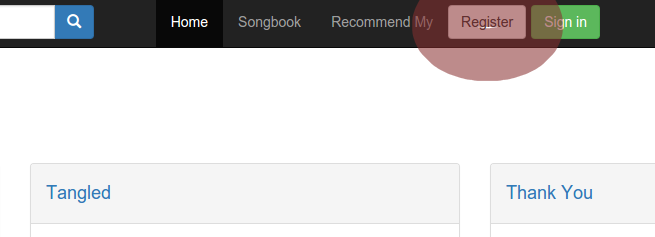
\includegraphics[scale=0.55]{tutorial_top_panel_register}
        \caption{Registrační tlačidlo}
        \label{fig:register_button}
    \end{center}
\end{figure}

\begin{figure}
    \begin{center}
        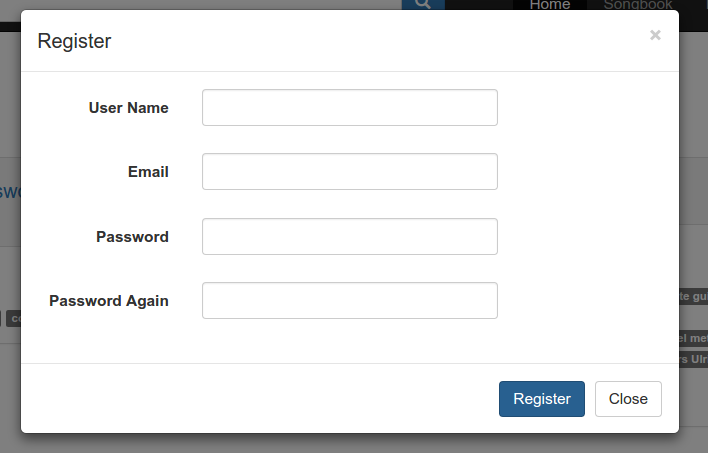
\includegraphics[scale=0.55]{register_form}
        \caption{Registračný formulár}
        \label{fig:register_form}
    \end{center}
\end{figure}

\subsection{Prihlásenie}

\begin{enumerate}
\item{Navigujeme sa na ktorúkoľvek podstránku aplikácie.}
\item{Kliknem na tlačitko Sign In vpravo hore.}
\item{Následne sa nám zobrazí registračný formulár \ref{fig:login_form}.}
\item{Vyplníme svoje prihlasovacie meno a heslo.}
\item{Klikne na Login.}
\item{Ak nenastala žiadna chyba mali by sme byť prihlásení.}
\end{enumerate}

\begin{figure}
    \begin{center}
        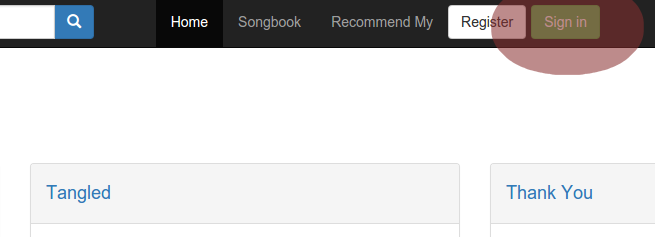
\includegraphics[scale=0.55]{tutorial_top_panel_login}
        \caption{Prihlasovacie tlačidlo}
        \label{fig:login_button}
    \end{center}
\end{figure}

\begin{figure}
    \begin{center}
        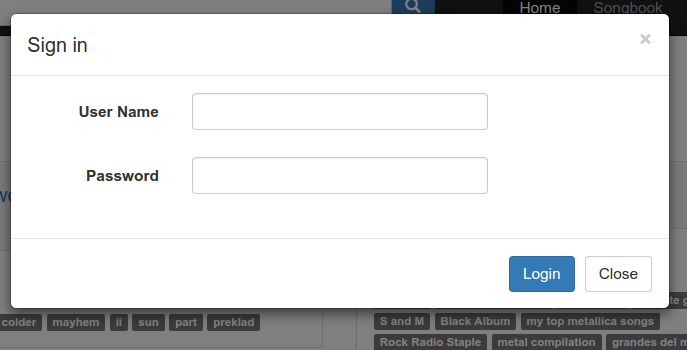
\includegraphics[scale=0.55]{login_form}
        \caption{Prihlasovací formulár}
        \label{fig:login_form}
    \end{center}
\end{figure}

\subsection{Vyhľadávanie}\label{sec:search}

Vyhľadáva sa pomocov textového poľa v hlavičke stránky \ref{fig:search_screen} (oblasť číslo 1),
ktoré je dostupné na každej podstránke. V prípade, že sa do nedá zadať vyhľadávací reťazec a
stlačí sa buď modrá lupa vpravo od poľa alebo enter, zobrazia sa výsledky ako na obrázku
\ref{fig:search_screen} (oblasť číslo 2).

\begin{figure}
    \begin{center}
        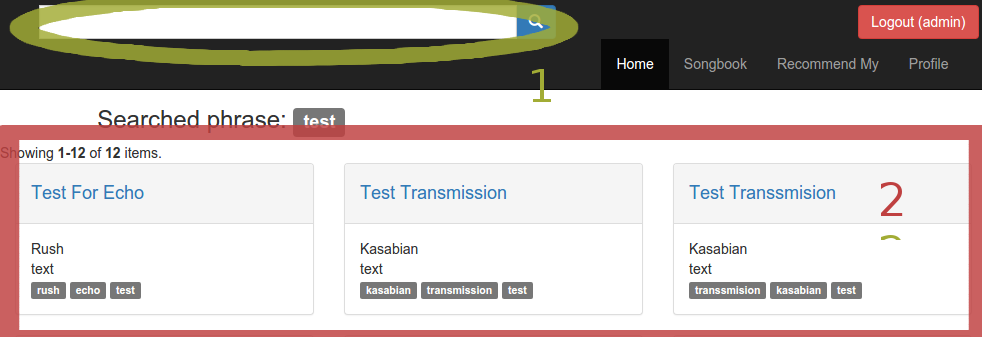
\includegraphics[scale=0.44]{search_screen}
        \caption{Vyhľadávacia obrazovka}
        \label{fig:search_screen}
    \end{center}
\end{figure}

\subsection{Vytvorenie spevníku}

\begin{enumerate}
\item{Klineme na tlačidlo Songbook v menu \ref{fig:songbook} (oblasť 1).}
\item{Zaškrtneme, pre ktorých používateľov chceme generovať spevník \ref{fig:songbook} (oblasť 2).}
\item{Kliknem na tlačidlo \uv{Create} \ref{fig:songbook} (oblasť 3).}
\item{Na obrázku \ref{fig:songbook} (oblasť 4) by mali byť zobrazené zoznamy odporúčaných
    piesni do spevníku.}
\end{enumerate}

\begin{figure}
    \begin{center}
        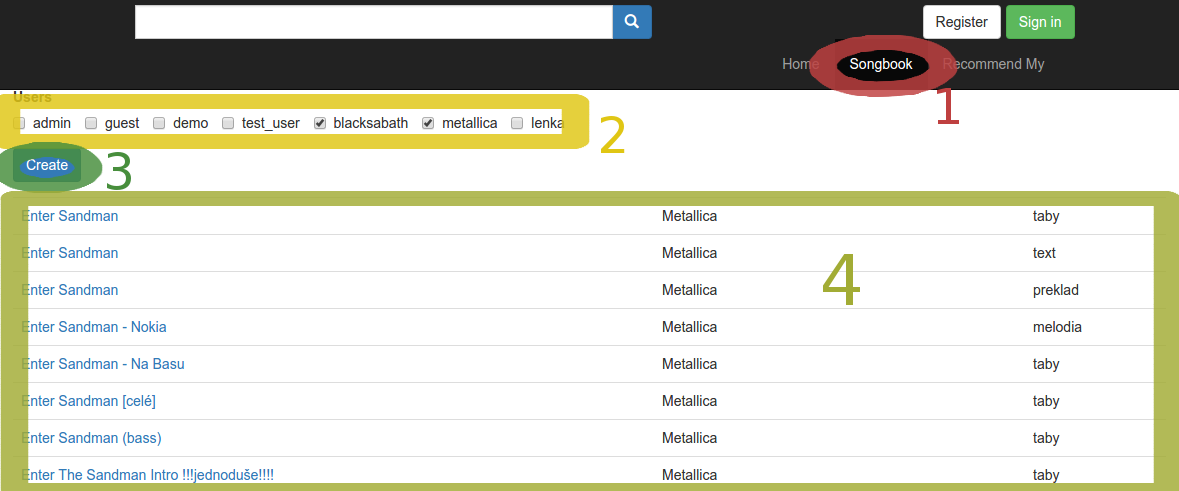
\includegraphics[scale=0.35]{obrazovka_songbook}
        \caption{Vyhľadávacia obrazovka}
        \label{fig:songbook}
    \end{center}
\end{figure}

\subsection{Zobrazenie odporúčaní}

Odporúčania sa zobrazujú na stránke v dvoch prípadoch. V prípade, že navštívite 
sekciu stránky \uv{Recommend My} alebo pri zobrazení dokumentu.

\subsubsection{Zobrazenie odporúčaní \uv{Recommend My}}

Na túto obrazovku sa dostaneme po kliknutí na \uv{Recommend My} v menu \ref{fig:recommendmy}
(oblasť 1). Na obrazovke sa následne nachádzajú dve tabuľky reprezentujúce dva rôzne algoritmy
na odporúčanie.

\begin{figure}
    \begin{center}
        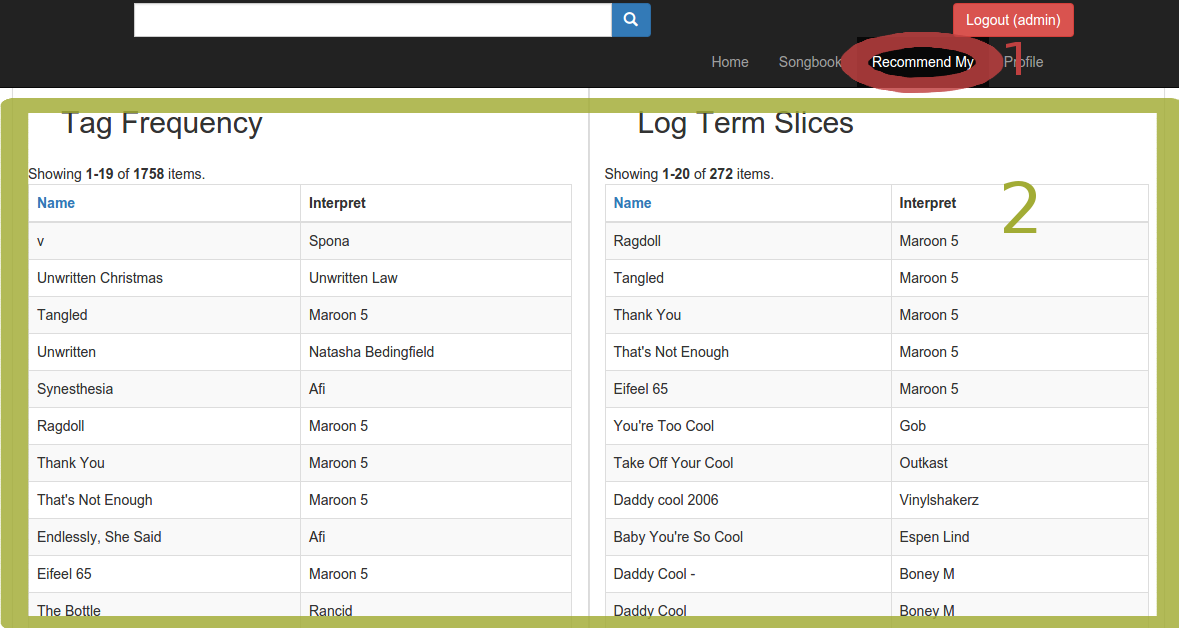
\includegraphics[scale=0.35]{recommend_my}
        \caption{Obrazovka odporúčaní}
        \label{fig:recommendmy}
    \end{center}
\end{figure}

\subsubsection{Zobrazenie odporúčaní pri zobrazení dokumentu}

Na túto obrazovku sa môžeme dostať buď z vyhľadávania opísanom vo Vyhľadávanie\ref{sec:search}.
Obrazovka obsahuje prvky:

\begin{itemize}
\item{Na obrázku \ref{fig:song} vľavo (oblasť 1) sa nachádza panel s tagmi dokumentu.}
\item{V strede (oblasť 2) sa nachádza aktuálny obsah dokumentu.}
\item{Vpravo hore (oblasť 3) je panel, ktorý zobrazuje dokumenty najviac podobné
    aktuálnemu dokumentu.}
\item{Vpravo dole (oblast 4) je panel, ktorý obsahuje odporúčania pre aktuálneho používateľa.}
\end{itemize}


\begin{figure}
    \begin{center}
        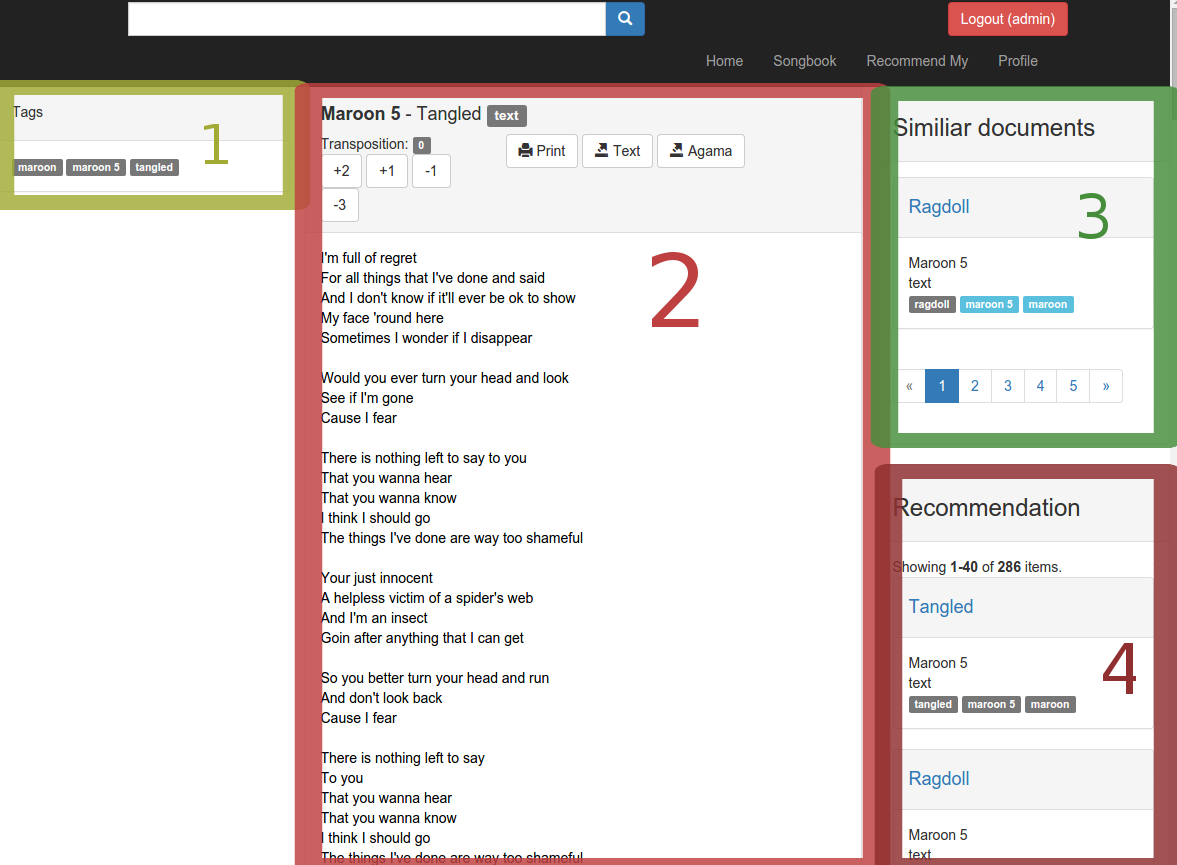
\includegraphics[scale=0.35]{song}
        \caption{Zobrazenie dokumentu}
        \label{fig:song}
    \end{center}
\end{figure}

\newpage

\subsection{Inštalačná príručka}\label{install_guide}

Zdrojové súbory sú na digitálnom nosiči v podpriečinku src/.
Aby aplikácia mohla fungovať, potrebuje z webu prístupný podpriečinok src/web a
potrebuje aby PHP skripty sa mohli zapisovať do priečinka src/runtime.

\paragraph{Kontrola minimálnych požiadaviek}

Pre presné stanovenie splnenia minimálnych požiadaviek je v 
priečinku so zdrojovými súbormi skript \uv{requirements.php}. Tento skript
je potrebné spustiť v konzole. Skript upozornení na prípadné možné 
problémy s kompatibilitou. Ak budú vypísané upozornenia znamená to, že aplikácia bude
fungovať, avšak v niektorých situáciach môže nastať nedefinovaný stav.

\paragraph{Inštalácia balíkov Composer-a}

Na nainštalovanie všetkých knižníc použitých pri vývoji a závislostiach aplikácie
je potrebne z koreňového priečinka inštalácie (priečinok src/) spustiť
príkaz \ref{lst:composer_install}. V pripade že nemáte nainštalovaný Composer,
môžete postupovať podľa oficiálneho návodu\footnote{https://getcomposer.org/doc/00-intro.md}.

\begin{lstlisting}[label=lst:composer_install, caption=Inštalácia balíkov Composer-a]
composer install
\end{lstlisting}

\paragraph{Inštalácia databázy}

Prvý krok na pripojenie k databáze je nastavenie prístupových parametrov databázy.
Tieto sa nastavujú v súbore \uv{src/config/db.php}. Príklad na nastavenie MySQL databázy
je v ukážke \ref{db_mysql} a príklad na nastavenie PostgreSQL je v ukážke \ref{db_postgres}.

\begin{lstlisting}[label=db_mysql,caption=Príklad nastavenia databázy MySQL]
<?php

return [
    'class' => 'yii\db\Connection',
    'dsn' => 'mysql:'.
            'host=localhost;'.
            'port=3303;'.
            'dbname=database',
    'username' => 'username',
    'password' => 'password',
    'charset' => 'utf8',
];
\end{lstlisting}

\begin{lstlisting}[label=db_postgres,caption=Príklad nastavenia databázy PostgreSQL]
<?php

return [
    'class' => 'yii\db\Connection',
    'dsn' => 'pgsql:'.
            'host=localhost;'.
            'port=5432;'.
            'dbname=database',
    'username' => 'username',
    'password' => 'password',
    'charset' => 'utf8',
    'schemaMap' => [
        'pgsql' => [
            'class' => 'yii\db\pgsql\Schema',
            'defaultSchema' => 'public',
        ]
    ]
];
\end{lstlisting}

Po nastavení pripojenia k databáze je treba ešte vytvoriť v databáze potrebnú štruktúru tabuliek.
Na spravovanie zmien v štruktúre databázy boli použité migrácie aplikačného rámca Yii2. 
Na vytvorenie tabuliek a cudzích kľučov stačí spustiť prikaz \uv{./yii migrate}
v koreňovom priečinku aplikácie (\uv{src/}).

\paragraph{Otestovanie funkčnosti súčiastok}

V prípade potreby je možné v tomto bode spustiť automatizované testovanie, čo však vyžaduje 
prítomnosť ďaľšej databázy (testovanie prepisuje základné dáta), prístupy k databáze pre 
tester sa nastavujú v súbore \uv{src/tests/codeception/config/config.php}.

Ďalej je potrebne spustiť migrácie, tento krát ich ale púšťame z priečinka \uv{src/tests}
a použijeme príkaz \uv{./codeception/bin/yii migrate}. Následne môžeme spustiť 
testy pomocov \uv{codecept run unit}. Aby testovanie fungovalo, vyžaduje sa aby v danom
prostredí bol nainštalovaný testovací aplikačný rámec
Codeception\footnote{http://codeception.com/install}.

\paragraph{Príkazy pre manažéra úloh}

Pokiaľ nechceme manuálne spúšťať indexovanie a prednačítanie externých databáz je dobré 
pridať tieto príkazy do manažéra úloh,

\begin{itemize}
\item{\textbf{./yii interpret/explore} - získava názvy a identifikátory interpretov zo stránok
    ktoré obsahuju zoznamy interpretov,}
\item{\textbf{./yii document/explore} - snaží sa získať identifikátory dokumentov,
    ich interpretov a typ,}
\item{\textbf{./yii document/parallelnametags} - paralelne vygeneruje značky
    z názvu dokumentu, názvu interpreta a typu dokumentu,
\item{\textbf{./yii document/lunloaded} - snaží sa stiahnuť obsahy dokumentov a značky
    z last.fm, tento príkaz sa dá spustiť aj paralelne ako
    \textbf{./yii document/parallelunloaded}, tento prístup však nemusí fungovať všade
    a nie je spoľahlivý,}
\item{\textbf{./yii mapdocumenttag/weight} - vypočítava užitočnosť značiek.}
\end{itemize}

Aplikácia obsahuje aj ďaľšie príkazy:

\begin{itemize}
\item{\textbf{./yii document/paralleltaglfm} - paralélne sťahuje značky z last.fm},
\item{\textbf{./yii document/tagtype \$id} - \$id je parameter identifikátor dokumentu,
    vygeneruje značky pre dokument z jeho názvu, názvu jeho interpreta a typu dokumentu,}
\item{\textbf{./yii document/tagtypes} - skontroluje, či všetky značky priradené dokumentom
    sú správneho typu, existuje aj paralelna verzia \textbf{./yii document/paralleltagtypes},}
\end{itemize}

\paragraph{Nastavenia}

Aplikácia po nainštalovaní bude bežať vo vývojovom móde. Pre produkčné nastavenie je 
potrebné zmeniť nastavenia v \uv{src/web/index.php}. V danom súbore je potrebné zmeniť
zakomentovať riadky 4 a 5 a odkomentovať riadky 8 a 9.

Ďalej aplikácia obsahuje nastavenia v súbore \uv{src/config/params.php}.

\begin{itemize}
\item{\textbf{tag\_appereance\_weights} - váhy jednotlivých domén značiek,}
\item{\textbf{min\_tag\_lenght} - minimálna dĺžka slova aby sa mohlo stať značkou,}
\item{\textbf{time\_aware\_recomendation} - ak je nastavený na \uv{true}, pri zobrazení
    piesne sa na paneli z odporúčaniami zobrazujú výsledky nášho algoritmu, ak
    je hodnota \uv{false}, zobrazujú sa výsledky agregačného algoritmu.}
\end{itemize}

\section{Elektronické médium}

K dokumentu priložené elektronické médium má nasledovnú štruktúru:
\begin{my_itemize}

\emptyitem /doc
    \begin{my_itemize}
    \myitem bakalárska práca spolu s anotáciami v slovenskom a anglickom jazyku
    \end{my_itemize}

\emptyitem /src/doc
    \begin{my_itemize}
    \myitem súbor s referenciami vo formáte BibTeX a súbory dokumentácia vo formáte Latex
    \end{my_itemize}

\emptyitem /src
    \begin{my_itemize}
    \myitem zdrojové kódy samotnej implementovanej aplikácie
    \end{my_itemize}

\emptyitem readme.txt
    \begin{my_itemize}
    \myitem popis obsahu média v slovenskom a anglickom jazyku
    \end{my_itemize}
\end{my_itemize}

